\subsection{Descripci\'on del problema}

Somos parte de una empresa que provee soluciones algorítmicas para problemas sobre redes informáticas. Tenemos un cliente que desea implementar un servicio particular en una red de computadoras ya existente.
Partiendo de esta, lo que desea es crear una red de computadoras, donde debe haber un backbone de servidores el cuál debe tener una topología de red de tipo anillo, manteniendo conectadas (de forma directa o indirecta) a este backbone a todas las demás computadoras de la red.
Todo esto debe realizarse minimizando a nivel óptimo el costo total de las conexiones de la red.

Por ejemplo en la siguiente imágen mostramos una posible red de nuestro cliente.

\begin{figure}[H]
\begin{center}
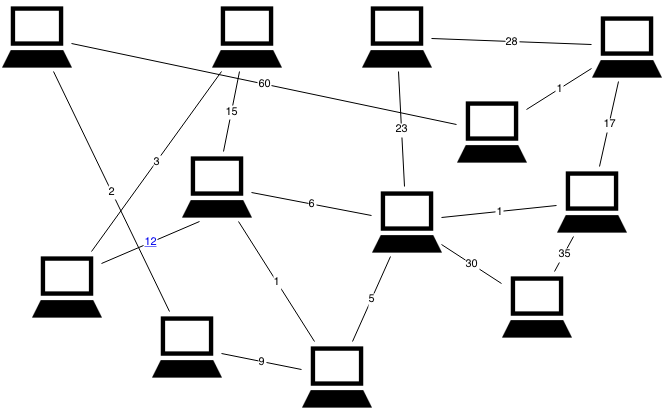
\includegraphics[scale=.35]{./imagenes/ej3_ejemplo1.png}
\caption{Red inicial.}
\end{center}
\end{figure}

Y a continuación se puede ver como debería quedar la red. El anillo formado se muestra con dos conexiones solo para resaltarla.

\begin{figure}[H]
\begin{center}
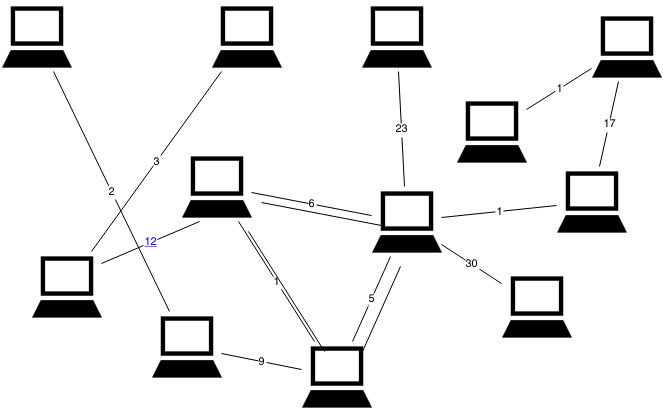
\includegraphics[scale=.35]{./imagenes/ej3_ejemplo2.png}
\caption{Modelo final de red, con un backbone tipo anillo.}
\end{center}
\end{figure}

\newpage

%%%%%%%%%%%%%%%%%%%%%%%%%%%%%%%%%%%%%%%%%%%%%%%%%%%%%%%%%%%%%%%%%%%%%%%%%%%%%%%%%%%%%%%%%%%%%%%%%%%%%%%%%%%%%%%%%%%%%%%%%%%%%%%%%%%%%%%%%%%%%%%%%%%%%%%%%%%%%%%%%%%%%%%%%%%%%%%%%%%%%%%%%%%%%%%%%%%%%%%%%%%%%%%%%%%%%%%%%%%%%%%%%%%%%%%%%%%%%%%%%%%%%%%%%%%%%%%%%%%%%%%%%%%%%%%%%%%%%%%%%%%%%%%%

\subsection{Resoluci\'on}

Para resolver el problema observamos la gran similitud, o igualdad en todo caso, entre:
El problema de crear una red de tipo anillo y conectar toda una serie de computadoras a esta de manera de minimizar el costo de conexión, utilizando para esto un conjunto de conexiones entre todas las computadoras, ya existente.
Y el problema de obtener de un grafo G, exactamente una componente conexa con al menos un circuito, de manera de minimizar el peso total de las aristas. Razón por la cual pensamos que la mejor forma de resolver el problema era obtener un árbol generador mínimo a partir de las computadoras y sus conexiones, para así llegar a tener todas las computadoras conectadas entre sí. Luego agregar la conexión de menor costo que no se haya usado para así crear la red de servidores tipo anillo.
Una vez obtenido el anillo buscamos y contamos las conexiones que pertenecen a \'el.
Para obtener la red de computadoras (el \'arbol generador m\'inimo) utilizamos el algoritmo de Kruskal, algo modificado, para que tambi\'en devuelva la conexi\'on de menor costo no utilizada, preferimos Kruskal sobre el algoritmo de Prim simplemente por gusto. Para buscar las conexiones pertenecientes al anillo utilizamos el algoritmo BFS, con el cu\'al podemos obtener el camino m\'inimo (en realidad \'unico ya que se ejecuta sobre un \'arbol) en un tiempo lineal.
A modo de ejemplo agregamos un pseudo-código del algoritmo propuesto:

\begin{itemize}
\item resolver($conexiones$)
\item Obtengo un AGM $agm$ y la menor conexion $c$ que queda fuera con Kruskal de $conexiones$.
\item Busco el anillo $A$ con bfs desde una computadora de $c$ a la otra.
\item Busco el conjunto de conexiones $C$ que pertenecen a $agm$ pero no a $A$.
\item Imprimo $A$ y luego $C$.
\end{itemize}


\newpage

%%%%%%%%%%%%%%%%%%%%%%%%%%%%%%%%%%%%%%%%%%%%%%%%%%%%%%%%%%%%%%%%%%%%%%%%%%%%%%%%%%%%%%%%%%%%%%%%%%%%%%%%%%%%%%%%%%%%%%%%%%%%%%%%%%%%%%%%%%%%%%%%%%%%%%%%%%%%%%%%%%%%%%%%%%%%%%%%%%%%%%%%%%%%%%%%%%%%%%%%%%%%%%%%%%%%%%%%%%%%%%%%%%%%%%%%%%%%%%%%%%%%%%%%%%%%%%%%%%%%%%%%%%%%%%%%%%%%%%%%%%%%%%%%

\subsection{Demostraci\'on de la resoluci\'on}

Para demostrar que nuestra resoluci\'on realmente resuelve el problema propuesto haremos una demostraci\'on por partes.

Como ya dijimos, a grandes razgos la forma que proponemos de resolver el problema es correr el algoritmo de Kruskal para obtener un \'arbol generador mínimo (AGM) a partir de todas las conexiones ya existentes, y luego agregarle a este la conexión de menor costo que no haya sido utilizada. Con lo cual obtenemos el anillo que pasaría a ser parte del anillo de servidores.

Para demostrar que con este procedimiento efectivamente obtenemos una red con un backbone de servidores de tipo anillo y como efectivamente tratamos a este problema como un problema de grafos, a part\'ir de ahora diremos que las computadoras y servidores son nodos en el grafo, y las conexiones entre ellos serán las aristas, donde el costo de conexión es el peso de estas. Por lo tanto reducimos el problema a obtener un grafo de peso mínimo en el que todos los nodos formen solo una componente conexa y en esta exista un (y solo un) ciclo.

Ahora para ser mas claros separaremos la demostraci\'on en dos partes:

\begin{itemize}
\item Demostraremos que al obtener un AGM y agregarle la men\'or arista restante del grafo, obtenemos una componente conexa con \'un ciclo, de peso total óptimo.
\item Para demostrar lo anterior necesitaremos probar que no existe la posibilidad de que nuestra soluci\'on genere un AGM y pueda existir otro AGM que deje afuera a una arista de menor peso, siendo finalmente una soluci\'on mejor. Por lo tanto en segundo lugar probaremos que cualquier AGM de un mismo grafo siempre esta formado el mismo multiconjunto de pesos de aristas, por lo tanto la arista de menor peso que quede afuera de nuestro AGM siempre será del mismo peso (aunque pueda no ser la misma arista).
\end{itemize}

Por un simple hecho de comodidad comenzaremos demostrando el segundo punto:

Sean $T_1$ y $T_2$ dos AGM del grafo $G$, sean $M_1$ y $M_2$ los conjuntos de aristas que forman $T_1$ y $T_2$ respectivamente. Vamos a suponer que los multiconjuntos que forman los pesos de las aristas en $M_1$ y $M_2$ son distintos. Sea $W$ el conjunto de aristas que pertenece a $M_1$ y no a $M_2$, y viceversa. $\forall$ $x$ $\in$ $W$, ($x$ $\in$ $M_1$ $\wedge$ $x$ $\notin$ $M_2$) $\vee$ ($x$ $\in $$M_2$ $\wedge$ $x$ $\in$ $M_1$).
Tomamos de $W$ la arista de menor peso, la llamaremos $e$, y sin perdida de generalidad diremos que $e$ $\in$ $T_1$ $\wedge$ $e$ $\notin$ $T_2$. Podemos decir entonces que todas las aristas que posean menor peso que el de $e$ est\'an en $T_1$ y en $T_2$.
Como $T_2$ es un AGM si le agregamos una arista, se formar\'a un ciclo que la contiene, llamemoslo $C$. Ahora podemos observar que en este ciclo $C$ debe existir al menos una arista $e'$ tal que $e'$ $\notin$ $T_1$, porque sino ser\'ia lo mismo que decir que en $T_1$ hay un ciclo, y esto no es posible ya que es un AGM. Tambi\'en podemos decir que le peso de $e'$ es mayor o igual al peso de $e$ por la observaci\'on hecha anteriormente, y aqu\'i pueden pasar dos cosas:
\begin{itemize}
\item $e'$ $\geq$ $e$
\end{itemize}
Si $e'$ $\geq$ $e$  entonces podr\'iamos agregar $e$ a $T_2$ y sacar $e'$, finalmente formando un \'arbol $T_3$ de peso menor que el de $T_2$. Esto es absurdo ya que $T_2$ era un AGM, y no podr\'ia haber un \'arbol de peso menor.

\begin{itemize}
\item $e'$ $=$ $e$
\end{itemize}
Si $e'$ $=$ $e$, podr\'iamos agarrar la arista de menor peso en $W$ $\setminus$ $e$  y repetir el procedimiento.

Como supusimos que los pesos de las aristas en $M_1$ y $M_2$ son distintos, en alg\'un momento debemos llegar a formar un ciclo en $T_2$ tal que en el existe una arista $e'$ de peso mayor que el de $e$, de otra forma W estar\'ia formado por pares de aristas de un mismo peso donde una pertenece a $T_1$ y otra a $T_2$, o dicho de otra forma, los multiconjuntos que forman los pesos de las aristas que est\'an fuera de cada AGM son iguales, lo que implica que los multiconjuntos de pesos de aristas que estos forman tambi\'en son iguales, y esto tambi\'en ser\'ia absurdo, ya que supusimos que estos multiconjuntos de $M_1$ y $M_2$ son distintos.

Ahora que sabemos que un AGM est\'a formado siempre por un conjunto de aristas de los mismos pesos, podemos decir que al tener el conjunto de aristas total $C_1$ y le sacamos las aristas del AGM $C_2$, $C_1$ tambi\'en estar\'a formado por un conjunto de aristas de los mismos pesos para cualquier AGM. Por lo tanto podemos asegurar que la arista de menor peso que queda afuera puede no ser siempre la misma, pero siempre ser\'a del mismo peso.

Con esto podemos demostrar el primer punto:

Como sabemos, por definici\'on un \'arbol generador de un grafo $G$ es un \'arbol que tiene el mismo conjunto de nodos que $G$, y un \'arbol generador mínimo es un \'arbol generador tal que el peso total (o longitud) de las aristas es el mínimo posible.
Por lo tanto si queremos tener todas las computadoras conectadas entre s\'i, es normal pensar que queremos tener todos los nodos en una misma componente conexa.
Al mismo tiempo pensamos en un AGM, porque no existe otra forma de tener conectados todos los nodos de un grafo minimizando el peso, sin que este sea un \'arbol, si este no es un arbol es porque tiene alg\'un ciclo, entonces podr\'iamos sacar cualquier arista de ese ciclo y finalmente obtendr\'iamos un grafo de peso menor.

Finalmente si conectamos todos los nodos mediante un AGM, podemos decir que es la forma de tener a todos conectados minimizando el peso total de las aristas. Si queremos generar un ciclo en este grafo, solo bastaría con agregar la arista de menor peso que haya quedado fuera del arbol y aquí el porque de la demostracion anterior. Ahí confirmamos que sin importar que AGM me genere Kruskal, la arista de menor peso que quede afuera siempre tendr\'a el mismo peso, por lo tanto no podr\'ia existir otro AGM que me deje una arista de peso menor afuera y finalmente este forme una soluci\'on mejor.

Por lo tanto podemos confirmar que obteniendo un AGM y agregandole la arista de menor peso que haya quedado fuera obtenemos una componente conexa con un (y solo un) ciclo tal que el peso total de las aristas sea m\'inimo.


\newpage

%%%%%%%%%%%%%%%%%%%%%%%%%%%%%%%%%%%%%%%%%%%%%%%%%%%%%%%%%%%%%%%%%%%%%%%%%%%%%%%%%%%%%%%%%%%%%%%%%%%%%%%%%%%%%%%%%%%%%%%%%%%%%%%%%%%%%%%%%%%%%%%%%%%%%%%%%%%%%%%%%%%%%%%%%%%%%%%%%%%%%%%%%%%%%%%%%%%%%%%%%%%%%%%%%%%%%%%%%%%%%%%%%%%%%%%%%%%%%%%%%%%%%%%%%%%%%%%%%%%%%%%%%%%%%%%%%%%%%%%%%%%%%%%%

\subsection{Complejidad del algoritmo}

La complejidad del algoritmo la plantearemos a partir de varios pseudo-códigos:

\begin{itemize}
\item Complejidad de Kruskal
\item Complejidad de BFS para obtener las aristas pertenecientes al ciclo
\item Complejidad del algoritmo final
\end{itemize}

\subsubsection{Complejidad Kruskal}


\begin{itemize}
\item $KRUSKAL$
\item Me creo un grafo, $AGM$, vacío donde iré guardando el árbol generador mínimo creado.
\item Para cada vértice $v$ en $G$. $O(n)$
\begin{itemize}
	\item Creo un conjunto de pertenencia. $O(1)$
\end{itemize}
\item Mientras no haya agregado $n-1$ aristas y no revise todas las aristas (recorriendo las aristas en orden ascendente segun su peso). $O(m.log(n))$ $\footnote{reference: Introduction to Algorithms 3er ed. - Cormen, Leiserson, Rivest, Stein - pag. 633}$
\begin{itemize}
	\item Si $a$ y $b$ no pertenecen al mismo conjunto de pertenencia (donde $a$ y $b$ son los nodos que conecta la arista $v$). $O(1)$
	\begin{itemize}
		\item Agrego la arista a $AGM$. $O(1)$
		\item Actualizo el conjunto de pertenencia de $b$ y todos los nodos adyacentes a el. $O(n)$ 
		\item Sumo 1 a la cantidad de aristas agregadas. $O(1)$
	\end{itemize}
	\item Sino, Si aun no encontre la primer arista excluida del árbol. $O(1)$
	\begin{itemize}
		\item Me guardo la arista excluida. $O(1)$
	\end{itemize}
\end{itemize}
\item devuelvo $AGM$
\end{itemize}


\subsubsection{Complejidad BFS}

\begin{itemize}

\item bfs(agm G, vertice inicio, vertice fin)
\item Para cada vértice $u$ en $G-{inicio}$. $O(n)$
\begin{itemize}
	\item Seteo $u$ como no visitado, distancia = infinito y predecesor = nulo. $O(1)$
\end{itemize}
\item Seteo $inicio$ como visitado, distancia 0 (cero), predecesor nulo. $O(1)$
\item Creo una cola $Q$ y encolo $inicio$. $O(1)$
\item Mientras la cola no este vacía. $O(n)$ 
\begin{itemize}
	\item Desencolo un elemento $s$.
	\item Para cada vértice $v$ adjacente a $s$. $O(n)$
	\begin{itemize}
		\item Si no visite $v$:
        \begin{itemize}
			\item Marco distancia de $v$ = distancia de $s + 1$, predecesor = $s$.
			\item Encolo $v$.
			\item Si $v$ = $fin$, termino.
        \end{itemize}
	\end{itemize}
	\item Marco $s'$ como visitado
\end{itemize}
\end{itemize}

La complejidad real de bfs es $O(n + m)$ $\footnote{reference Introduction to Algorithms 3er ed. - Cormen, Leiserson, Rivest, Stein - pag. 597}$ (m = $\#$aristas, n = $\#$vertices). Pero en este caso decimos que la complejidad de BFS es $O(n)$ porque siempre se ejecutará sobre \'arboles. 


\subsubsection{Complejidad del algoritmo}


\begin{itemize}
\item resolver($conexiones$)
\item Obtengo un AGM $agm$ y la menor conexion $c$ que queda fuera con Kruskal de $conexiones$. $O(m.log(n))$
\item Busco el anillo $A$ con bfs desde una computadora de $c$ a la otra. $O(n)$
\item Busco el conjunto de conexiones $C$ que pertenecen a $agm$ pero no a $A$. $O(n)$ (*)
\item Imprimo $A$ y luego $C$.
\end{itemize}

(*) Aquí podemos decir que la complejidad es $O(n)$ porque solo recorremos las conexiones del árbol que son $n$.

Como se puede observar el algoritmo tiene una complejidad acotada por $O(m.log(n))$


\newpage

%%%%%%%%%%%%%%%%%%%%%%%%%%%%%%%%%%%%%%%%%%%%%%%%%%%%%%%%%%%%%%%%%%%%%%%%%%%%%%%%%%%%%%%%%%%%%%%%%%%%%%%%%%%%%%%%%%%%%%%%%%%%%%%%%%%%%%%%%%%%%%%%%%%%%%%%%%%%%%%%%%%%%%%%%%%%%%%%%%%%%%%%%%%%%%%%%%%%%%%%%%%%%%%%%%%%%%%%%%%%%%%%%%%%%%%%%%%%%%%%%%%%%%%%%%%%%%%%%%%%%%%%%%%%%%%%%%%%%%%%%%%%%%%%

\subsection{C\'odigo fuente}

\lstset{language=C++,
                basicstyle=\ttfamily\footnotesize,
                keywordstyle=\color{blue}\ttfamily,
                stringstyle=\color{red}\ttfamily,
                commentstyle=\color{green}\ttfamily,
                morecomment=[l][\color{magenta}]{\#},
                breaklines=true
}
\begin{lstlisting}

MatrizAdyacencia kruskal(int cantCompus, int cantTotalAristas, Red& red, Enlace& menorEnlaceExcluido){
    Red redOrdenada = red;
    MatrizAdyacencia agm(cantCompus);
    vector<int> pertenece(cantCompus); // indica a que arbol pertenece el nodo
 
    for(int i = 0; i < cantCompus; i++){
        agm[i] = vector<int> (cantCompus, 0);
        pertenece[i] = i;
    }
 
    int compu1, compu2, costo;
    int cantAristas = 1;
    int posicionEnRed = 0;
    int cantAristasVisitadas = 0;

    bool noEncontreEnlaceExcluido = true;

    while(cantAristas < cantCompus && cantAristas <= cantTotalAristas){
        compu1 = redOrdenada[posicionEnRed].compu1;
        compu2 = redOrdenada[posicionEnRed].compu2;
        costo = redOrdenada[posicionEnRed].costo;
        posicionEnRed++;
        cantAristasVisitadas++;

        if(pertenece[compu1] != pertenece[compu2]){
            agm[compu1][compu2] = costo;
            agm[compu2][compu1] = costo;
 
        	int temp = pertenece[compu2];
        	pertenece[compu2] = pertenece[compu1];
        	for(int k = 0; k < cantCompus; k++)
        		if(pertenece[k] == temp)
        			pertenece[k] = pertenece[compu1]; 
            cantAristas++;
        }else{
            if(noEncontreEnlaceExcluido){
                menorEnlaceExcluido.compu1 = compu1;
                menorEnlaceExcluido.compu2 = compu2;
                menorEnlaceExcluido.costo = costo;
                noEncontreEnlaceExcluido = false;
            }
        }
    }
    return agm;
}





\end{lstlisting}


\newpage

%%%%%%%%%%%%%%%%%%%%%%%%%%%%%%%%%%%%%%%%%%%%%%%%%%%%%%%%%%%%%%%%%%%%%%%%%%%%%%%%%%%%%%%%%%%%%%%%%%%%%%%%%%%%%%%%%%%%%%%%%%%%%%%%%%%%%%%%%%%%%%%%%%%%%%%%%%%%%%%%%%%%%%%%%%%%%%%%%%%%%%%%%%%%%%%%%%%%%%%%%%%%%%%%%%%%%%%%%%%%%%%%%%%%%%%%%%%%%%%%%%%%%%%%%%%%%%%%%%%%%%%%%%%%%%%%%%%%%%%%%%%%%%%%

\subsection{Casos de prueba}

En este ejercicio decidimos hacer los casos de prueba con las siguientes caracter\'isticas:

\begin{itemize}
\item Caso en el que las conexiones todas las conexiones dadas no forman una sola red conjunta. De esta forma el algoritmo no tiene solución, por lo cual debería devolver "no".
\item Caso con los costos de todas las conexiones distintos. En este caso se devería observar que las conexiones que forman la red son las $n$ conexiones de menor costo, donde $n$ es la cantidad de computadoras de la red.
\item 
\end{itemize}


\newpage

%%%%%%%%%%%%%%%%%%%%%%%%%%%%%%%%%%%%%%%%%%%%%%%%%%%%%%%%%%%%%%%%%%%%%%%%%%%%%%%%%%%%%%%%%%%%%%%%%%%%%%%%%%%%%%%%%%%%%%%%%%%%%%%%%%%%%%%%%%%%%%%%%%%%%%%%%%%%%%%%%%%%%%%%%%%%%%%%%%%%%%%%%%%%%%%%%%%%%%%%%%%%%%%%%%%%%%%%%%%%%%%%%%%%%%%%%%%%%%%%%%%%%%%%%%%%%%%%%%%%%%%%%%%%%%%%%%%%%%%%%%%%%%%%

\subsection{Performance}

Para realizar el testeo de performance de nuestro algoritmo creamos el archivo 'test.cpp' en el cu\'al generamos instancias de prueba variando pseudo-aleatoriamente la cantidad de computadoras y conexiones, y su distribuci\'on.
En la generación de casos no discriminamos entre aquellos que tienen soluci\'on y los que no, pero por como es nuestro algoritmo, aquellos casos que no tienen soluci\'on terminarán mucho antes, por lo que los tiempos de ejecuci\'on de estos se graficarán apartadamente.

Primero modificaremos un poco el archivo test.cpp para que genere varias instancias con el mismo n\'umero de computadoras pero variando la cantidad de conexiones para ver la influencia de esta en el tiempo de ejecuci\'on.

%ANALISIS DE ESTE CASO




